\section{Semaine 25 (28/04 - 02/05) }


\e{Notions abordées :}
\begin{itemize}
	\item Mouvements à forces centrales (cf semaine précédente).
	\item Diagrammes E-pH.
	\item Mécanique du solide.
\end{itemize}

\subsection{Questions de cours}

\begin{enumerate}
	\item Théorème de la résultante dynamique.
	\item Définir le moment d'inertie d'un solide par rapport à un axe. Dimension et signification physique.
	\item Théorème du moment cinétique pour un solide en rotation autour d'un axe fixe.
\end{enumerate}

\subsection{Exercice 1 : Diagramme $E-pH$ du molybdène}

Le diagramme potentiel-pH du système molybdène-eau est présenté ci-dessous. Il est limité aux espèces les plus stables \ce{Mo}, \ce{Mo^{3+}}, \ce{MoO2}, \ce{MoO3}, \ce{HMoO4^-} et \ce{MoO4^{2-}}.

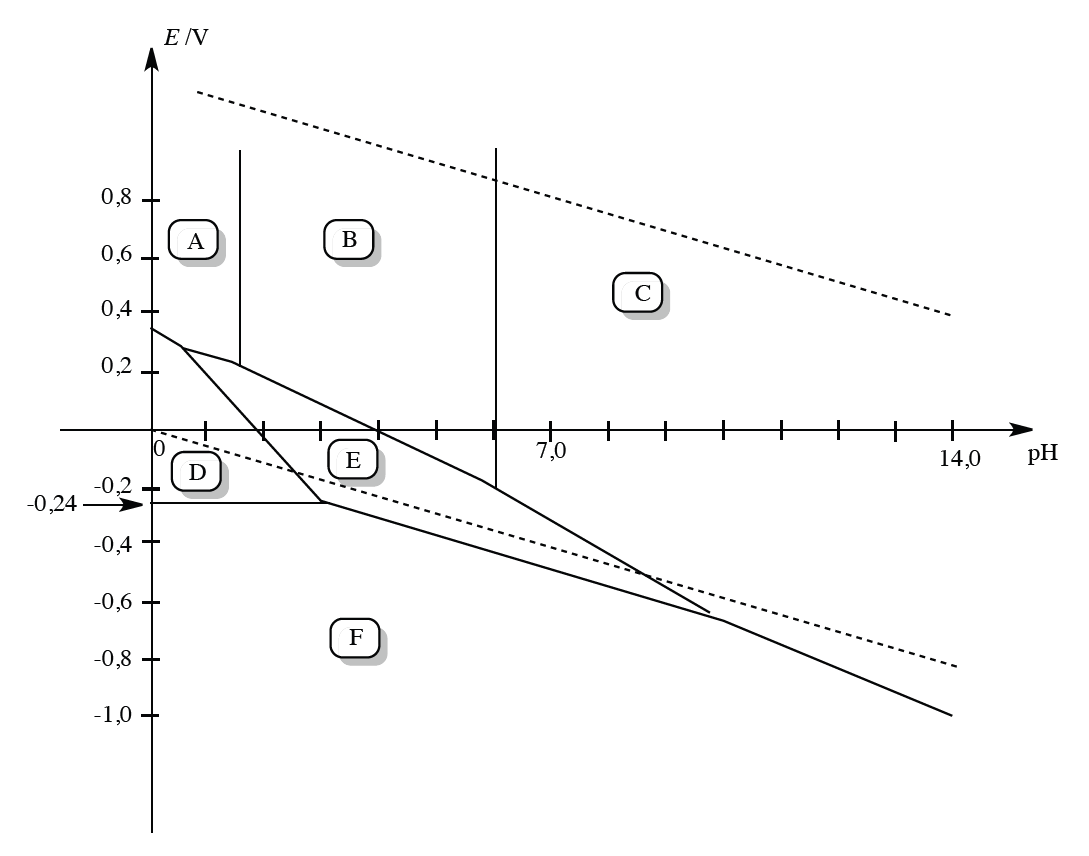
\includegraphics[width=\textwidth]{Images/mpsi_s25_ex01.png}

Les conventions adoptées pour le tracé de ces diagrammes sont les suivantes :
\begin{itemize}
	\item La concentration totale en élément molybdène est égale à $c_{tot}$.
	\item À la frontière qui sépare les domaines de deux espèces dissoutes, les concentrations en éléments \ce{Mo} dans chacune des espèces sont les mêmes.
\end{itemize}

\begin{enumerate}
	\item Proposer des états de la matière pour chacune des espèces.
	\item Placer les espèces dans le diagramme potentiel-pH en précisant le type de domaine à chaque fois (existence ou prédominance).
	\item Déduire du diagramme la valeur approchée de la concentration utilisée $c_{tot}$. Déduire de même la constante d'acidité du couple acido-basique impliquant l'ion \ce{MoO4^{2-}}.
	\item Le diagramme potentiel-pH de l'eau est représenté en pointillés. Rappeler les équation des droites qui le composent en utilisant, et rappelant, les conventions habituelles.
	\item Que se passe-t-il si on ajoute une base forte à une solution aqueuse désaérée (pas de dioxygène dissout) d'une suspension de dioxyde de molybdène ? Écrire les équations-bilans correspondantes.
\end{enumerate}

\e{Données :} $E^\circ(\ce{Mo^3+}/\ce{Mo}) = \SI{-0.20}{\volt}$

\e{Réponses :}
\begin{enumerate}
	\item -
	\item -
	\item $c_{tot} = \SI{1.0e-2}{\mol\per\liter}$ et $pK_A = \SI{6.0}{}$.
	\item -
	\item -
\end{enumerate}

\subsection{Exercice 2 : Mélange d'acide chlorhydrique et d'eau de Javel}

On dit souvent qu'il ne faut pas mélanger les produits ménagers, c'est en particulier le cas de l'eau de Javel avec tout produit à base d'acide. Essayons de comprendre pourquoi. Le gaz dichlore est un gaz toxique irritant, pouvant entraîner des problèmes pulmonaires graves en cas d'inhalation. L'eau de Javel est une solution aqueuse comportant du chlorure de sodium et de l'hypochlorite de sodium (\ce{NaClO} dissout) en quantité équimolaire. Le diagramme potentiel-pH simplifié du chlore est représenté ci-dessous, pour les espèces chimiques \ce{HClO_{(aq)}}, \ce{ClO^-_{(aq)}}, \ce{Cl2_{(aq)}} et \ce{Cl^-_{(aq)}} et pour une concentration de travail $c_T = \SI{0.1}{\mol\per\liter}$ en élément chlore.

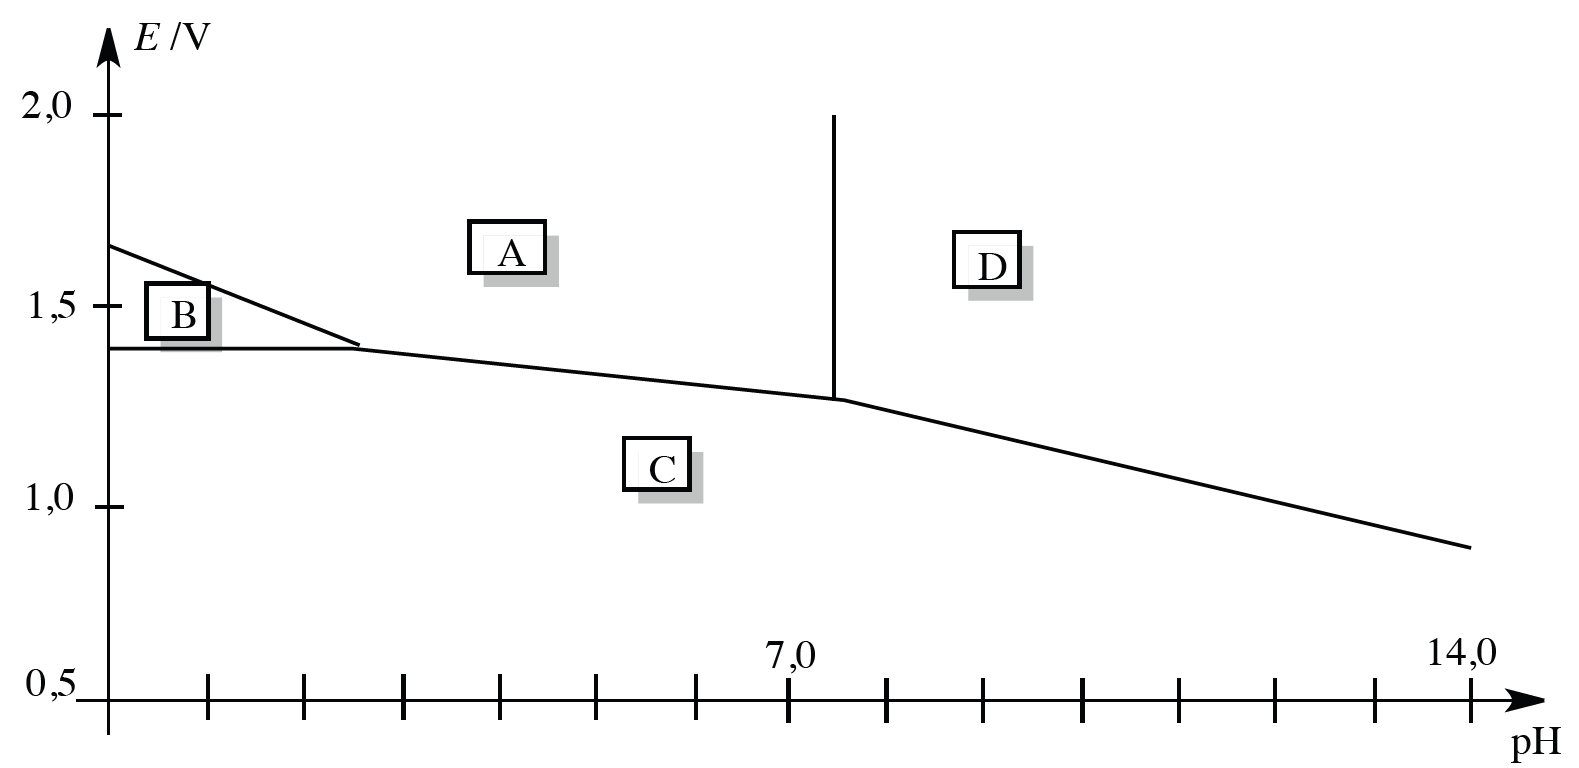
\includegraphics[width=\textwidth]{Images/mpsi_s25_ex02.png}

\begin{enumerate}
	\item À l'aide du diagramme potentiel-pH, retrouver la valeur du $pK_A$ du couple acido-basique composé d'espèces à même nombre d'oxydation. Tracer le diagramme de prédominance de ce couple. Quelle est l'espèce prédominante en milieu acide ?
	\item Placer les espèces chimiques mentionnées dans le diagramme potentiel-pH.
	\item En utilisant le diagramme potentiel-pH, prévoir l'évolution d'un mélange contenant les espèces $A$ et $C$ lors du passage en milieu très acide.
	\item En s'aidant des deux demi-équations électroniques relatives aux couples $A/B$ et $B/C$, écrire l'équation de la réaction entre les espèces $A$ et $C$ en milieu très acide.
	\item Comment appelle-t-on la réaction mise en jeu entre les espèces $A$ et $C$ ? Calculer sa  constante d'équilibre à $\SI{298}{K}$.
	\item Conclure quant à la consigne de sécurité figurant sur les flacons d'eau de Javel de ne pas mélanger un acide et de l'eau de Javel.
\end{enumerate}

\e{Données :} Pour les deux couples rédox comportant le dichlore, on donne $E^\circ_1 = \SI{1.39}{\volt}$ et $E^\circ_2 = \SI{1.60}{\volt}$.

\e{Réponse :} $K^\circ = 10^{3.5}$

\subsection{Exercice 3 : Diagramme potentiel-pH du plomb}

On donne le diagramme potentiel-pH simplifié du plomb, la concentration de tracé étant $c_T = \SI{1.0}{\mol\per\liter}$.

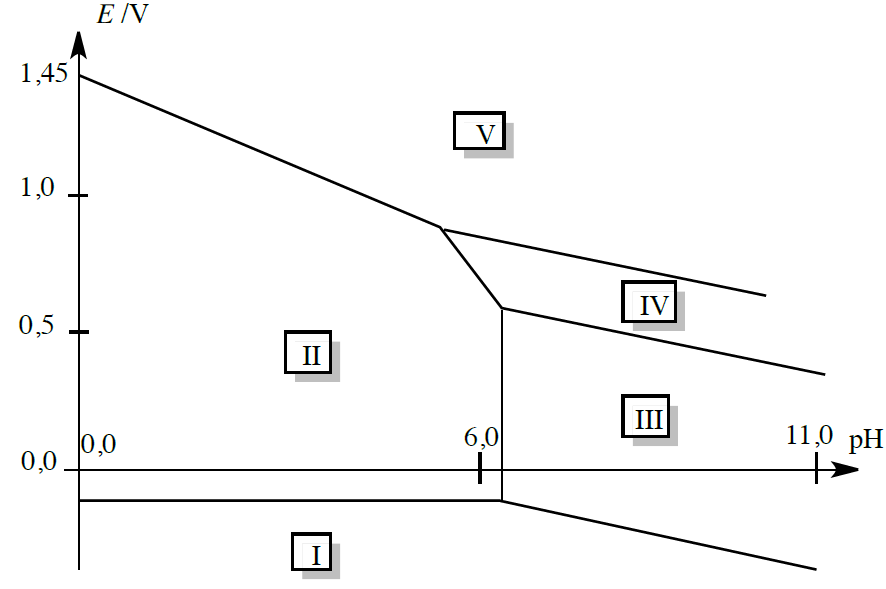
\includegraphics[width=\textwidth]{Images/mpsi_s25_ex03.png}

\begin{enumerate}
	\item Indiquer sur ce diagramme les domaines de prédominance ou d'existence des espèces suivantes : \ce{Pb^{2+}_{(aq)}}, \ce{Pb_{(s)}}, \ce{PbO_{(s)}}, \ce{PbO2_{(s)}} et \ce{Pb3O4_{(s)}}.
	\item Déterminer le potentiel standard du couple \ce{PbO2 / Pb^2+} par lecture du diagramme potentiel-pH. Donner l'équation numérique de la frontière entre ces espèces.
	\item Reproduire le diagramme puis le superposer au diagramme usuel de l'eau. 
	\item Que peut-on dire de la stabilité du plomb en solution aqueuse ? Discuter en fonction du $pH$ de la solution.
	\item Quelle réaction se produit entre le plomb et le dioxyde de plomb en milieu acide ? Comment nomme-t-on une telle réaction ?
\end{enumerate}

\e{Données :} $E^\circ(\ce{Pb^{2+}_{(aq)} / Pb_{(s)}}) = \SI{-0.13}{\volt}$

\e{Réponse :} $E^\circ = \SI{1.45}{\volt}$.

